% Uncomment this to make slides with overlays:
%\documentclass[slides]{beamer}

% Uncomment these (but comment the above \documentclass line) to make handouts:
\documentclass[handout]{beamer}

% Uncomment these to have more than one slide per page
%\usepackage{pgfpages}
%\pgfpagesuselayout{2 on 1}[border shrink=5mm]
%\pgfpageslogicalpageoptions{1}{border code=\pgfusepath{stroke}}
%\pgfpageslogicalpageoptions{2}{border code=\pgfusepath{stroke}}

\usepackage[]{graphicx, color, hyperref}

\mode<presentation>
{
	%\usetheme[secheader]{Boadilla}
	%\usecolortheme[rgb={.835, .102,.169}]{structure}  
	\usetheme[width= 0cm]{Goettingen}
	%\setbeamercovered{transparent}
}
\setbeamertemplate{navigation symbols}{}
\setbeamertemplate{footline}[frame number]

\definecolor{blue2}{rgb}{0.278,0.278,0.729} 
\newcommand{\blue}[1]{\textcolor{blue2}{#1}}
\newcommand{\white}[1]{\textcolor{white}{#1}}
\newcommand{\red}[1]{\textcolor{red}{#1}}
\newcommand{\xbar}{\overline{x}}
\newcommand{\ybar}{\overline{y}}
\newcommand{\phat}{\widehat{p}}
\newcommand{\prob}{\mbox{Pr}}
\newcommand{\E}{\mathbb{E}}
\newcommand{\Var}{\mbox{Var}}
\newcommand{\cp}{\oplus}
\newcommand{\cm}{\circleddash}

\title{Lecture 6: Visualizing Numerical and Categorical Data}
\author{Chapter 1.6+1.7}
\date{}

\begin{document}
%------------------------------------------------------------------------------
\begin{frame}
\titlepage
\end{frame}
%------------------------------------------------------------------------------=


%------------------------------------------------------------------------------
\begin{frame}[fragile]
\frametitle{Goals for Today}

\begin{itemize}
\item Rule of thumb for standard deviations
\item Population vs sample mean/variance/standard deviations
\item Percentiles and Quartiles
\item Boxplots
\item Piecharts, barplots, mosaicplots
\end{itemize}

\end{frame}
%------------------------------------------------------------------------------


%------------------------------------------------------------------------------
\begin{frame}[fragile]
\frametitle{Rule of Thumb for Standard Deviations}

%
% Comment this
%
If the data distribution is bell-shaped, then 
\begin{itemize}
\item about \blue{$\frac{2}{3}$} of the data will be within one SD of the mean (book says 70\%).
\item about \blue{95\%} of the data will be within two SD.
\end{itemize}

\end{frame}
%------------------------------------------------------------------------------


%------------------------------------------------------------------------------
\begin{frame}[fragile]
\frametitle{Example}

\begin{columns}
\column{.5\textwidth}
\begin{center}
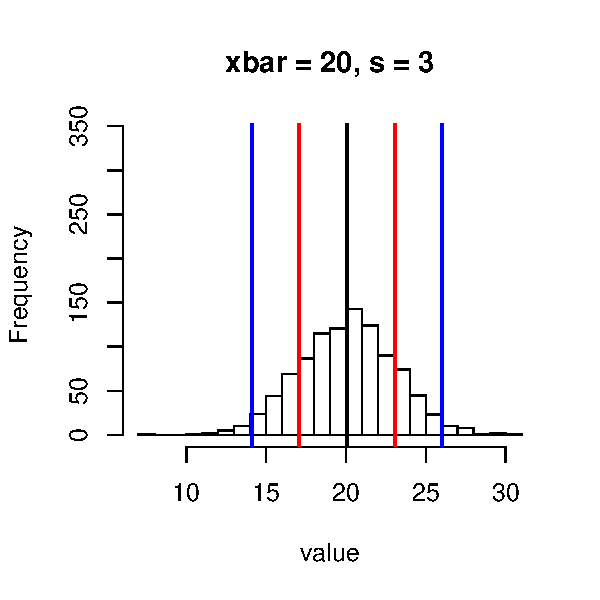
\includegraphics[width=\textwidth]{figure/spread3.pdf}
\end{center}
\column{.5\textwidth}
\begin{itemize}
\item black line is mean $\overline{x}$
\item red lines mark about $\frac{2}{3}$:  $[\overline{x} - s, \overline{x} + s] = [20 - 3, 20 + 3] = [17, 23]$.  
\item blue lines mark about 95\%: $[\overline{x} - 2s, \overline{x} + 2s] = [20 - 6, 20 + 6] = [14, 26]$.
\end{itemize}
\end{columns}

\end{frame}
%------------------------------------------------------------------------------


%------------------------------------------------------------------------------
\begin{frame}[fragile]
\frametitle{Population vs Sample Mean/Variance/Standard Deviation}

Recall the notion of taking a \blue{representative sample} from a \blue{study/target population}.  Say we are interested in the income of the individuals.   

\vspace{0.25cm}

\begin{center}
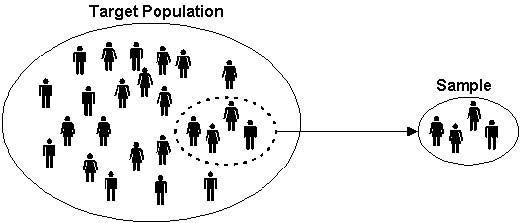
\includegraphics[width=3in]{figure/target-population.jpg} 
\end{center}


\end{frame}
%------------------------------------------------------------------------------


%------------------------------------------------------------------------------
\begin{frame}[fragile]
\frametitle{Population vs Sample Mean/Variance/Standard Deviation}
\begin{itemize}
\item The \blue{sample mean $\overline{x}$} is the mean income of the 4 sampled people.
\pause\item The \blue{population mean $\mu$} is the mean income of all 24 people in the target population.
\pause\item We say $\overline{x}$ \blue{estimates} $\mu$.  If the sample is representative, then $\overline{x}$ estimates $\mu$ with high \blue{accuracy} i.e. it is unbiased.
\end{itemize}

\end{frame}
%------------------------------------------------------------------------------


%------------------------------------------------------------------------------
\begin{frame}[fragile]
\frametitle{Population vs Sample Mean/Variance/Standard Deviation}

\begin{center}
  \begin{tabular}{r|cc}
	\hline	
     & True Population Value & Sample Value \\ 
	\hline	
    Mean & $\mu$ & $\overline{x}$ \\ 
    Variance & $\sigma^2$ & $s^2$ \\ 
    Standard Deviation & $\sigma$ & $s$ \\ 
	\hline	
  \end{tabular}
\end{center}

\pause The sample value is used to \blue{estimate} the (true) population value.  

\end{frame}
%------------------------------------------------------------------------------


%-------------------------------------------------------------------------------
\begin{frame}
\frametitle{Percentiles}
A percentile (\%'ile) indicates the value \blue{below} which a given \%'age of observations fall.  

\vspace{0.5cm}

\pause SAT Scores from 2012 \blue{\url{http://media.collegeboard.com/digitalServices/pdf/research/SAT-Percentile-Ranks-2012.pdf}}

\vspace{0.5cm}

\pause So for example, if you scored 700 in critical reading, 95\% of college-bound seniors who took the test did worse.

\end{frame}
%-------------------------------------------------------------------------------


%-------------------------------------------------------------------------------
\begin{frame}
\frametitle{Quartiles and IQR}

%
% Comment this
%
\blue{Quartiles} split up the data into 4 intervals, each with about one quarter of the data:

\vspace{0.25cm}

\begin{itemize}
\pause \item The lower quartile is the 25th \%'ile
\pause \item The median is the 50th \%'ile
\pause \item The upper quartile is the 75th \%'ile
\end{itemize}

\vspace{0.25cm}

\pause The \blue{interquartile range (IQR)} is another measure of the spread of a sample:
\[
\mbox{IQR} = \mbox{upper quartile} - \mbox{lower quartile}
\]

\end{frame}
%-------------------------------------------------------------------------------


%pdf("MLB_quartiles.pdf", width=8, height=6)
%hist(MLB$salary, breaks=seq(0, 35000, by=500), xlab="Annual Salary (in thousands of $)", main="Histograms of Major League Baseball Salaries")
%abline(v=summary(MLB$salary)[c(2,3,5)], col=c("red", "green", "blue"))
%legend("topright", legend=c("1st quartile", "2nd quartile", "3rd quartile"), 
%       col=c("red", "green", "blue"), lty=c(1,1, 1), lwd=2, bty='n')
%dev.off()
%-------------------------------------------------------------------------------
\begin{frame}[fragile]
\frametitle{MLB Data Quartiles}

\begin{verbatim}
 Min. 1st Qu.  Median    Mean 3rd Qu.    Max.
400.0   418.3  1094.0  3282.0  4250.0 33000.0
\end{verbatim}

\begin{center}
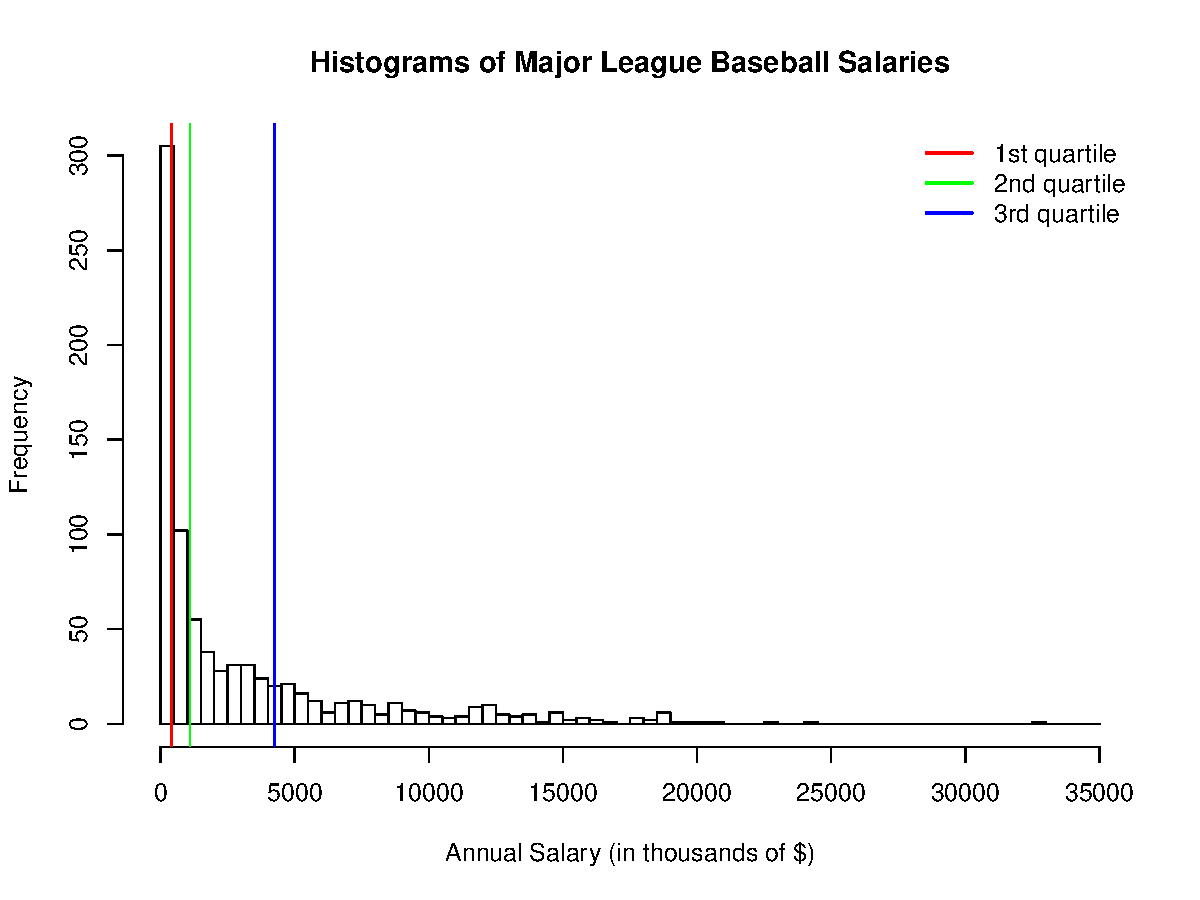
\includegraphics[height=5.5cm]{figure/MLB_quartiles.pdf}
\end{center}

The IQR is (3rd Quartile - 1st Quartile) = 4250.0 - 418.3 = 3831.7\\
i.e the distance between the red and blue line.  

\end{frame}
%-------------------------------------------------------------------------------


%-------------------------------------------------------------------------------
\begin{frame}
\frametitle{Robust Statistics (Chapter 1.6.6)}
\blue{Robust estimates} are statistics where extreme observations (outliers) have less effect on their values, i.e. are more resistant to their effect.  The median and IQR are two examples.  

\vspace{0.25cm}

\pause Example:  Old scoring system in figure skating: \blue{drop the highest \& lowest scores} and then take the average.  

\vspace{0.25cm}

\pause Say we have a figure skater who gets judged by countries V-Z:
\begin{center}
\begin{tabular}{r||ccccc}
\hline
Country & V & W & X & Y & Z \\ 
\hline
Score & 4.0 & 5.2 & 5.2 & 5.3 & 6.0 \\ 
\hline
\end{tabular}
\end{center}

\vspace{0.25cm}

\pause Drop the 4.0 and 6.0, then the final score is: $\frac{5.2 + 5.2 + 5.3}{3} = 5.23$
\end{frame}
%-------------------------------------------------------------------------------


%-------------------------------------------------------------------------------
\begin{frame}
\frametitle{Boxplots}
\blue{Boxplots} are visual summaries of a sample $x_1,\ldots,x_n$ that bring to light unusual values (potential outliers):

\vspace{0.5cm}

\pause Example: \# US Forces casualties in the war in Afghanistan for each month from 2008-2009:  

\vspace{0.5cm}

7, 1, 7, 5, 16, 28, 20, 22, 27, 16, 1, 3, 14, 15, 13, 6, 12, 24, 44, 51, 37, 59, 17, 17


\end{frame}
%-------------------------------------------------------------------------------


%pdf("afghanistan.pdf", width=8, height=4)
%casualties <- c(7, 1, 7, 5, 16, 28, 20, 22, 27, 16, 1, 3, 14, 15, 13, 6, 12, 24, 44, 51, 37, 59, 17, 17)
%boxplot(casualties, horizontal=TRUE, xlab="US Forces casualties in Afghanistan for each month 2008-2009")
%dev.off()
%summary(casualties)
%-------------------------------------------------------------------------------
\begin{frame}[fragile]
\frametitle{Boxplots}
\begin{verbatim}
Min. 1st Qu.  Median    Mean 3rd Qu.    Max. 
1.00    7.00   16.00   19.25   24.75   59.00 
\end{verbatim}
\begin{center}
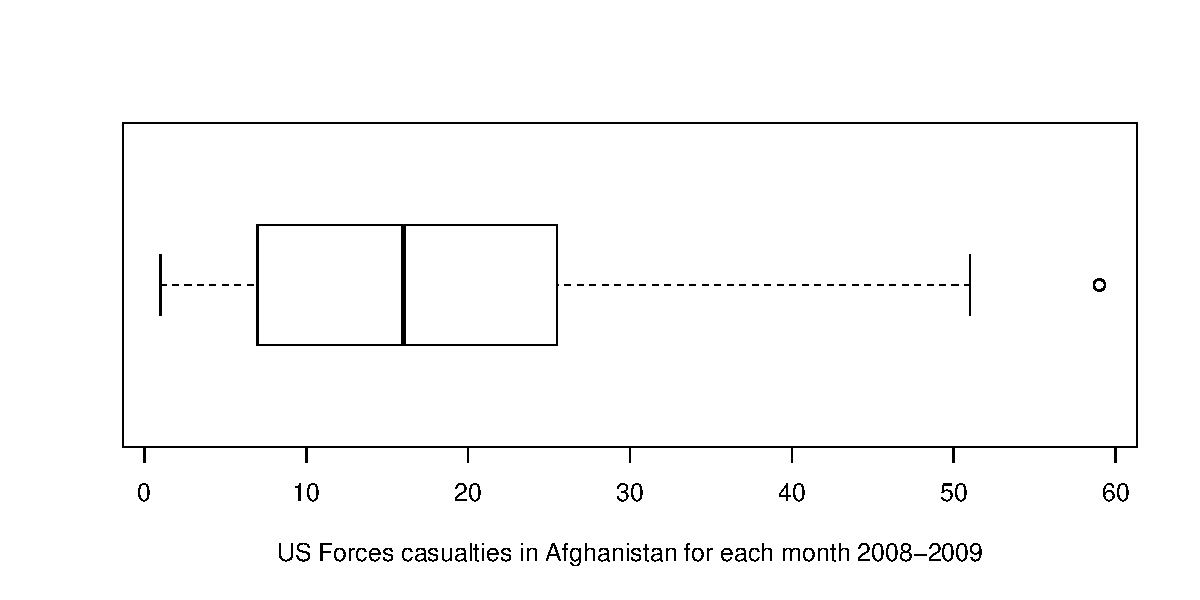
\includegraphics[height=4cm]{figure/afghanistan.pdf}
\end{center}
\pause Page 29 of text describes the length of the \blue{whiskers}: they capture data that is no more than $1.5 \times IQR$ of both ends of the box.  

\end{frame}
%-------------------------------------------------------------------------------


%-------------------------------------------------------------------------------
\begin{frame}
\frametitle{Outliers Are Relatively Extreme}
An \blue{outlier} is an observation that appears extreme relative to the rest of the data.

\vspace{0.5cm}

\pause Why it is important to look for outliers?  Examination of data for possible outliers serves many useful purposes, including
\begin{itemize}
\pause\item Identifying strong skew in the distribution.
\pause\item Identifying data collection or entry errors.
\pause\item Providing insight into interesting properties of the data.
\end{itemize}

\end{frame}
%-------------------------------------------------------------------------------


%------------------------------------------------------------------------------
\begin{frame}[fragile]
\frametitle{Piecharts}
Say we have the following piecharts represent the polling from a local election with five candidates (1-5) at three different time points A, B, an C:

\begin{center}
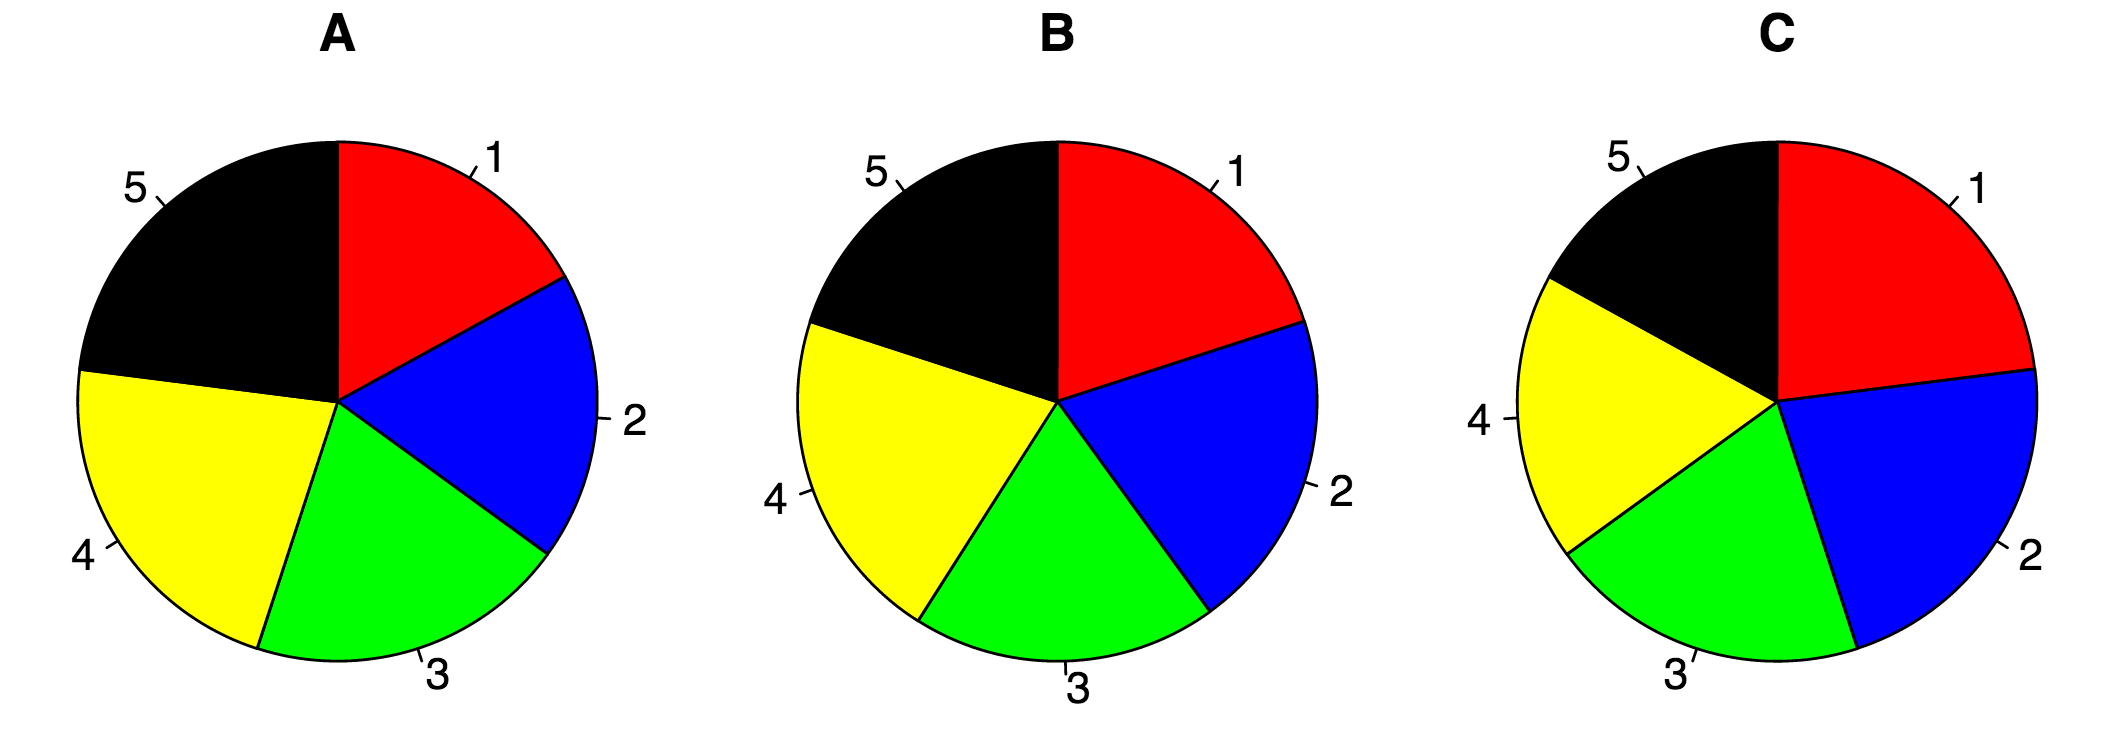
\includegraphics[width=\textwidth]{figure/piecharts.png}
\end{center}

\pause Answer the following questions:
\begin{itemize}
\item In the first race, is candidate 5 doing better than candidate 4?
\item Who did better between time A and time B, candidate 2 or candidate 4?
\end{itemize}

\end{frame}
%------------------------------------------------------------------------------


%------------------------------------------------------------------------------
\begin{frame}[fragile]
\frametitle{Barplots Instead}

\begin{center}
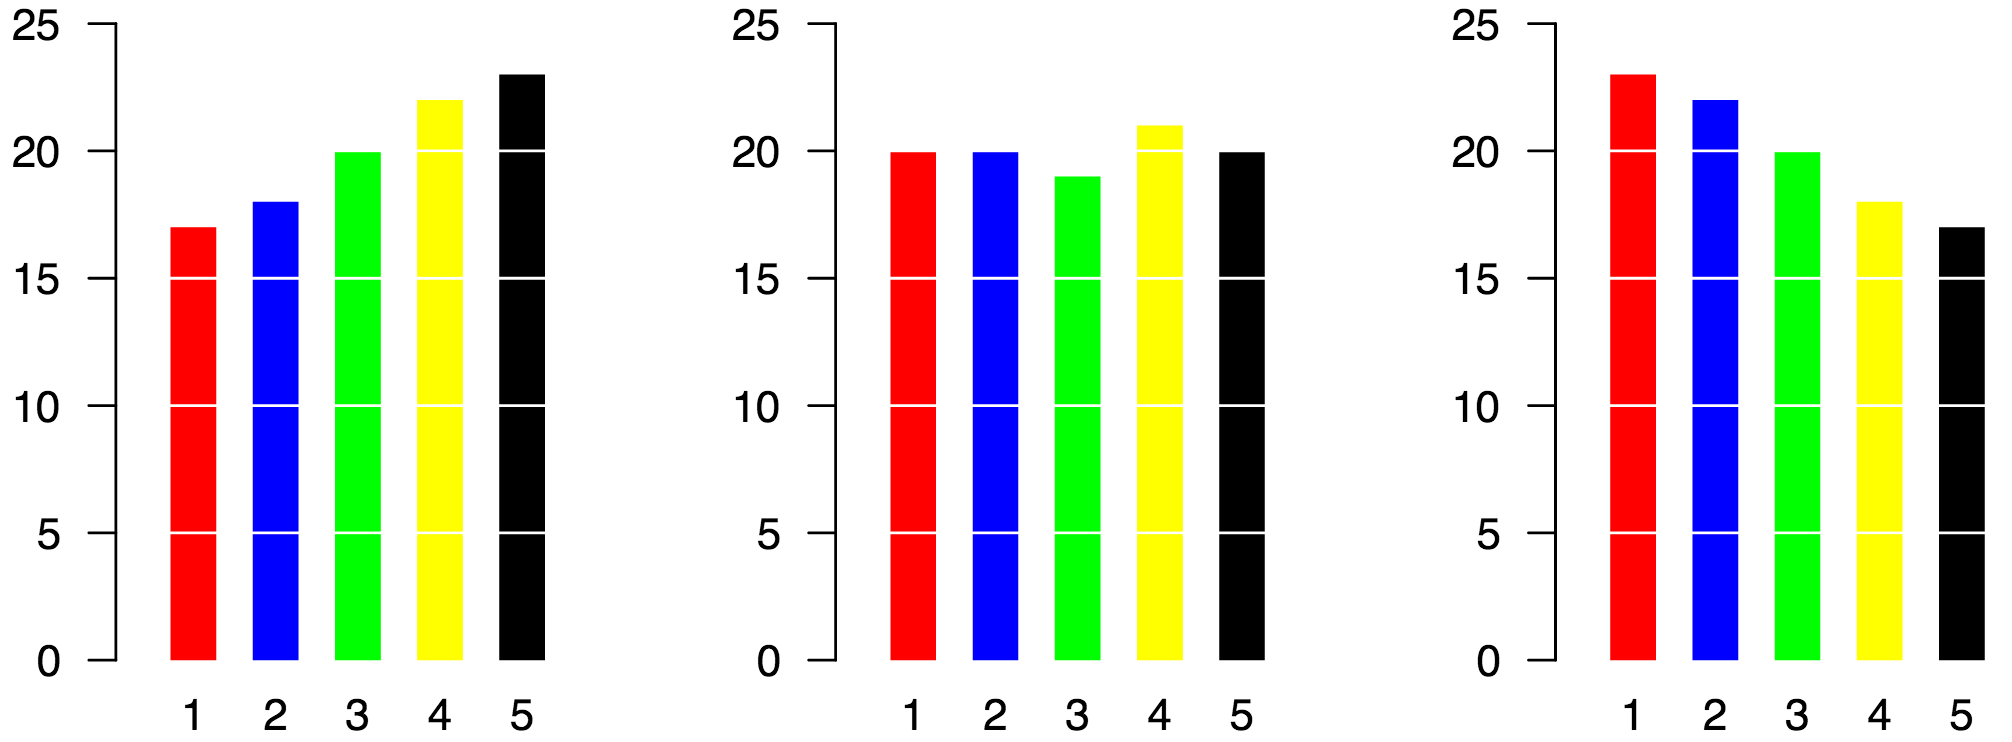
\includegraphics[width=\textwidth]{figure/barplots.png}
\end{center}

\vspace{0.5cm}

\pause Answers:
\begin{itemize}
\item Candidate 5 is doing better than 4
\item Between A and B, candidate 2 went from about 17\% to 20\% while candidate went from about 22\% to 21\%.  So candidate 2 did better
\end{itemize}

\end{frame}
%------------------------------------------------------------------------------


%------------------------------------------------------------------------------
\begin{frame}[fragile]
\frametitle{3D Piecharts Can Be Deceiving}

\begin{center}
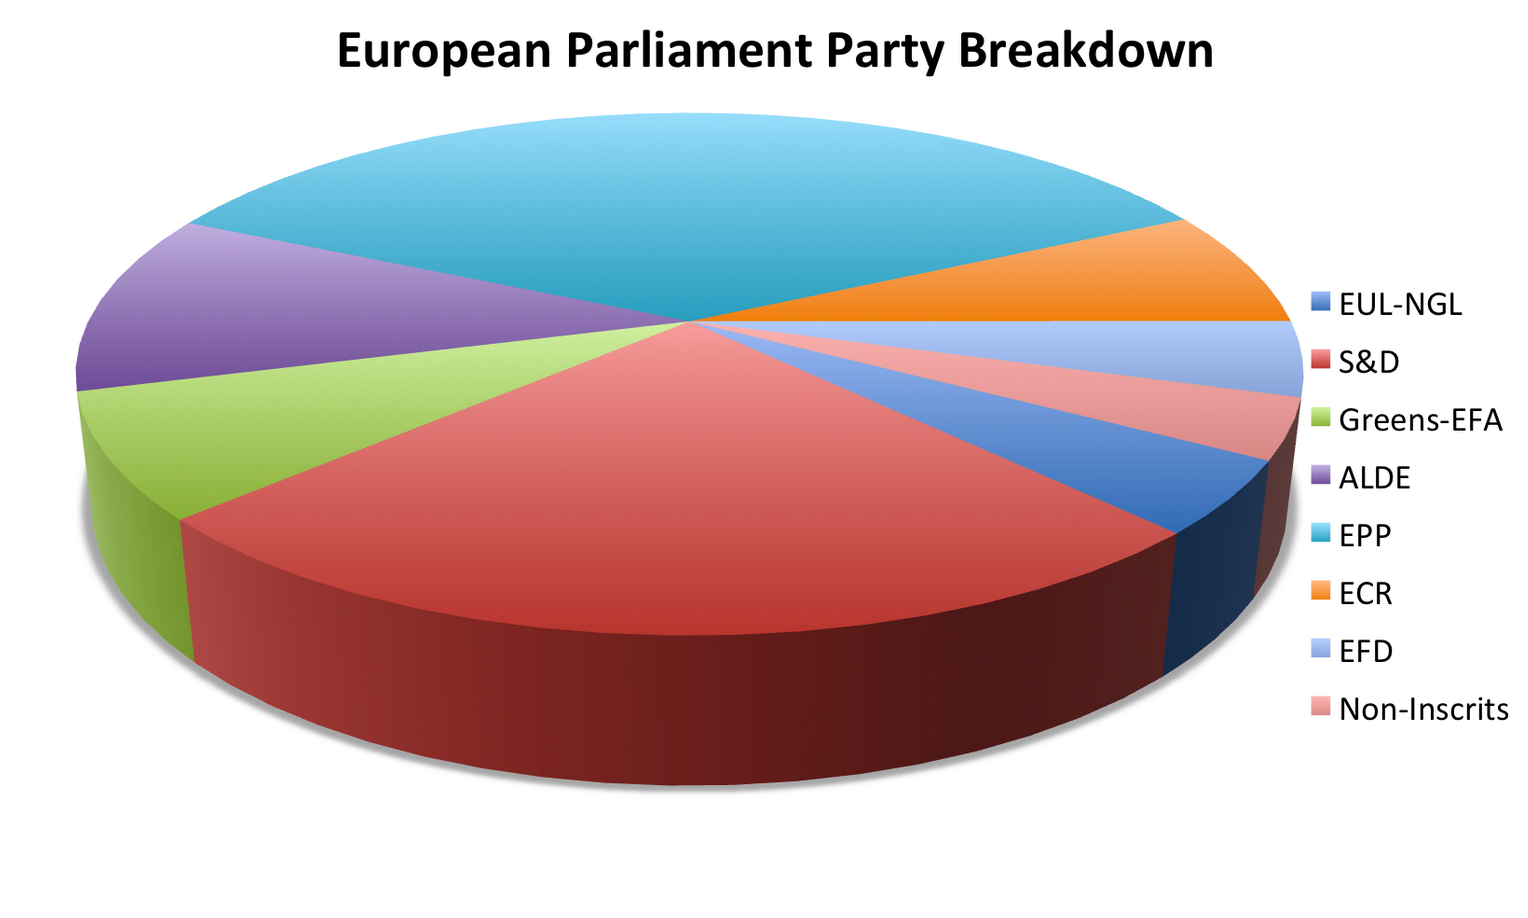
\includegraphics[width=\textwidth]{figure/europe.png}
\end{center}

EEP (teal) has 266 seats, whereas S\&D (red) has 190 seats.  


\end{frame}
%------------------------------------------------------------------------------


%------------------------------------------------------------------------------
\begin{frame}[fragile]
\frametitle{Titanic Survival Data}

Typing {\tt data(Titanic)} in R loads the survival and death counts, split by each of the following categories:

\pause \begin{itemize}
\item Class: 1st, 2nd, 3rd, or crew (4 levels)
\item Gender (2 levels)
\item Age: Child or adult (2 levels)
\end{itemize}

i.e. $4 \times 2 \times 2 = 16$ possible groups to consider.

\vspace{0.25cm}

Questions 

\begin{itemize}
\pause \item What was the effect of class (1st, 2nd, 3rd, crew) on your chances of survival?
\pause \item Did the ``women and children'' first lifeboat policy hold?
\end{itemize} 

\end{frame}
%------------------------------------------------------------------------------


%------------------------------------------------------------------------------
\begin{frame}[fragile]
\frametitle{Frequency Table}
A table summarizing a single categorial variable is called a \blue{frequency table}.  Overall:

\begin{center}
\begin{tabular}{r|rrrr|r}
Died & 1490 \\
  Survived & 711 \\  
   \hline
  Total & 2201 \\
\end{tabular}
\end{center}

\end{frame}
%------------------------------------------------------------------------------


%------------------------------------------------------------------------------
\begin{frame}[fragile]
\frametitle{Barplot}
\blue{Barplots} are ways to display categorial variables:

\begin{center}
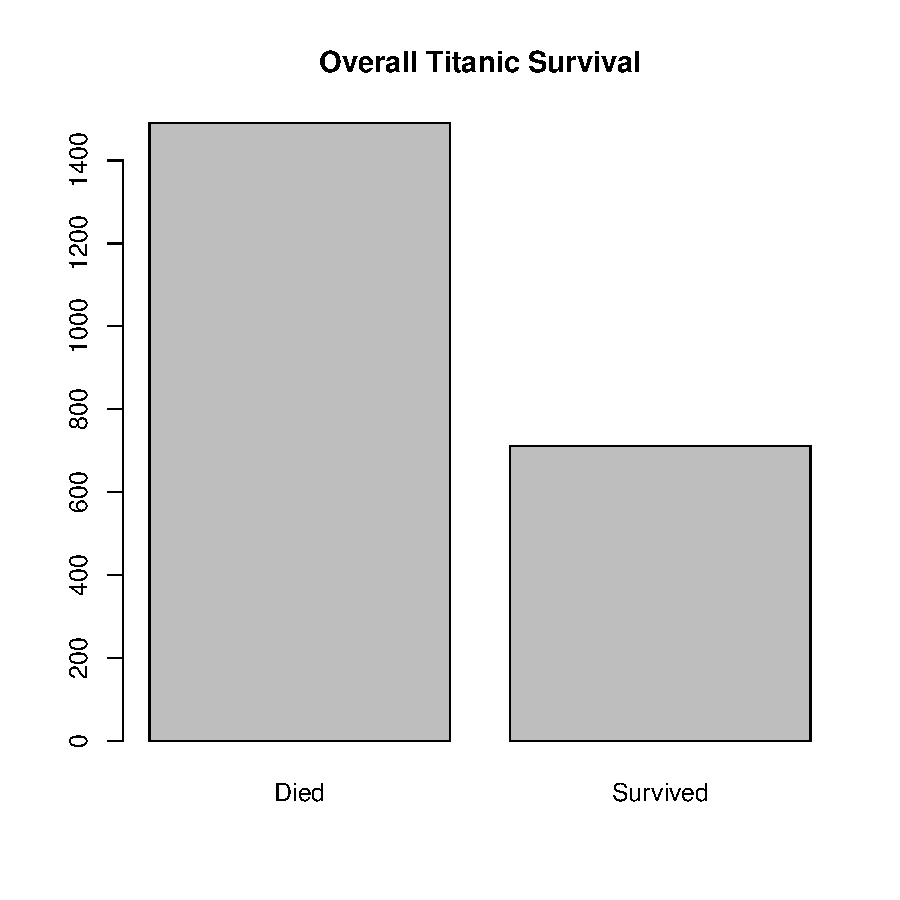
\includegraphics[width=5cm]{figure/barplot.pdf}
\end{center}


\end{frame}
%------------------------------------------------------------------------------


%------------------------------------------------------------------------------
\begin{frame}[fragile]
\frametitle{Contingency Table}
A table that \blue{cross-classifies} two categorical variables is a \blue{contingency table}.  Now let's split survival by class: 1st, 2nd, 3rd, and crew.

\pause \vspace{0.25cm}

Before:
\begin{center}
\begin{tabular}{r|rrrr|r}
Died & 1490 \\
  Survived & 711 \\  
   \hline
  Total & 2201 \\
\end{tabular}
\end{center}

After:
\begin{center}
\begin{tabular}{r|rrrr|r}
 & 1st & 2nd & 3rd & Crew & Total \\ 
  \hline
Died & 122 & 167 & 528 & 673 & 1490 \\ 
  Survived & 203 & 118 & 178 & 212 & 711 \\ 
   \hline
  Total & 325 & 285 & 706 & 885 & 2201 \\ 
\end{tabular}
\end{center}
  
\end{frame}
%------------------------------------------------------------------------------


%------------------------------------------------------------------------------
\begin{frame}[fragile]
\frametitle{Stacked Barplot}
\blue{Stacked barplots} are one way to display values from a contingency table:

\begin{center}
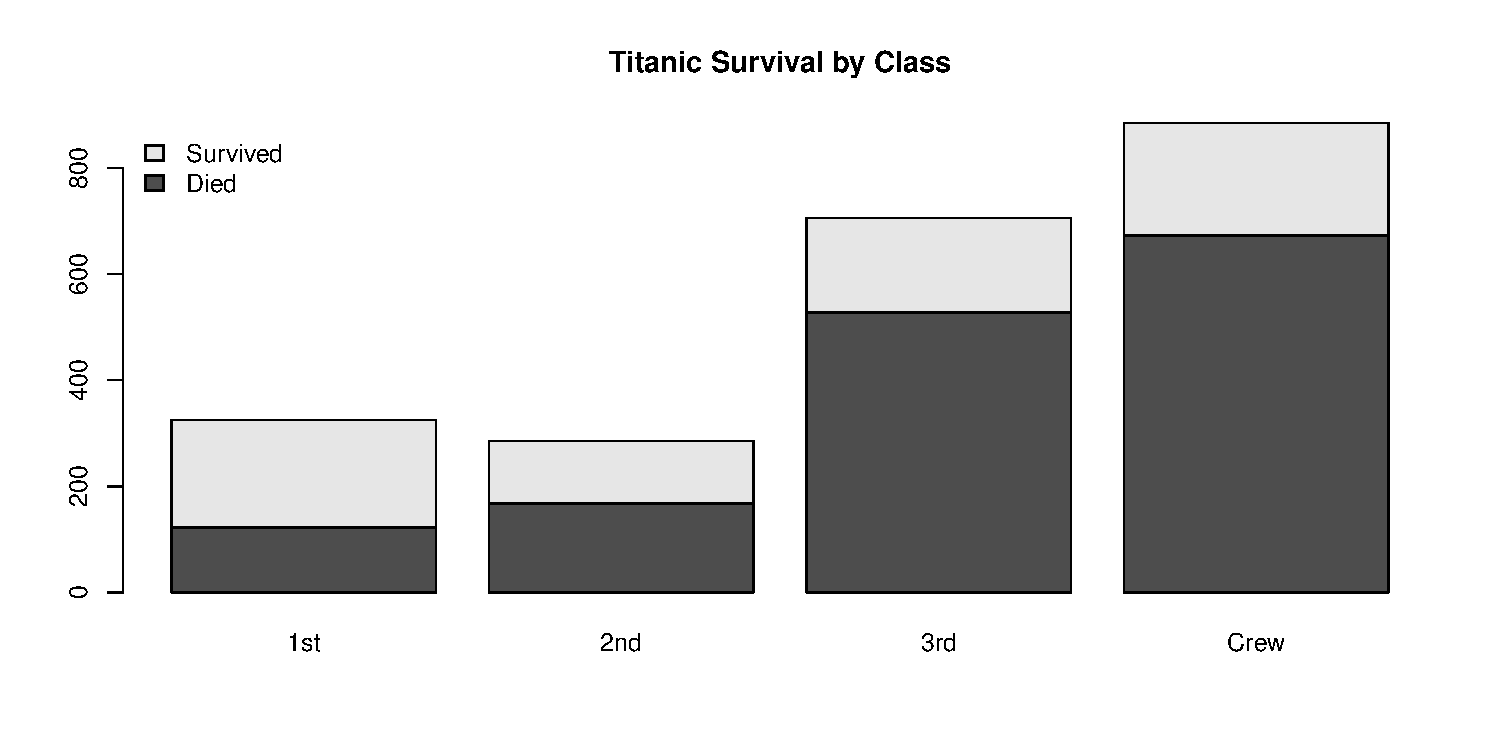
\includegraphics[width=10cm]{figure/barplot2.pdf}
\end{center}

\end{frame}
%------------------------------------------------------------------------------


%%------------------------------------------------------------------------------
%\begin{frame}[fragile]
%\frametitle{Standardized/Normalized Stacked Barplot}
%\blue{Standardized/normalized stacked barplots}:  Now show proportions in each bar, so that it is easier to compare across bars.  
%
%\begin{center}
%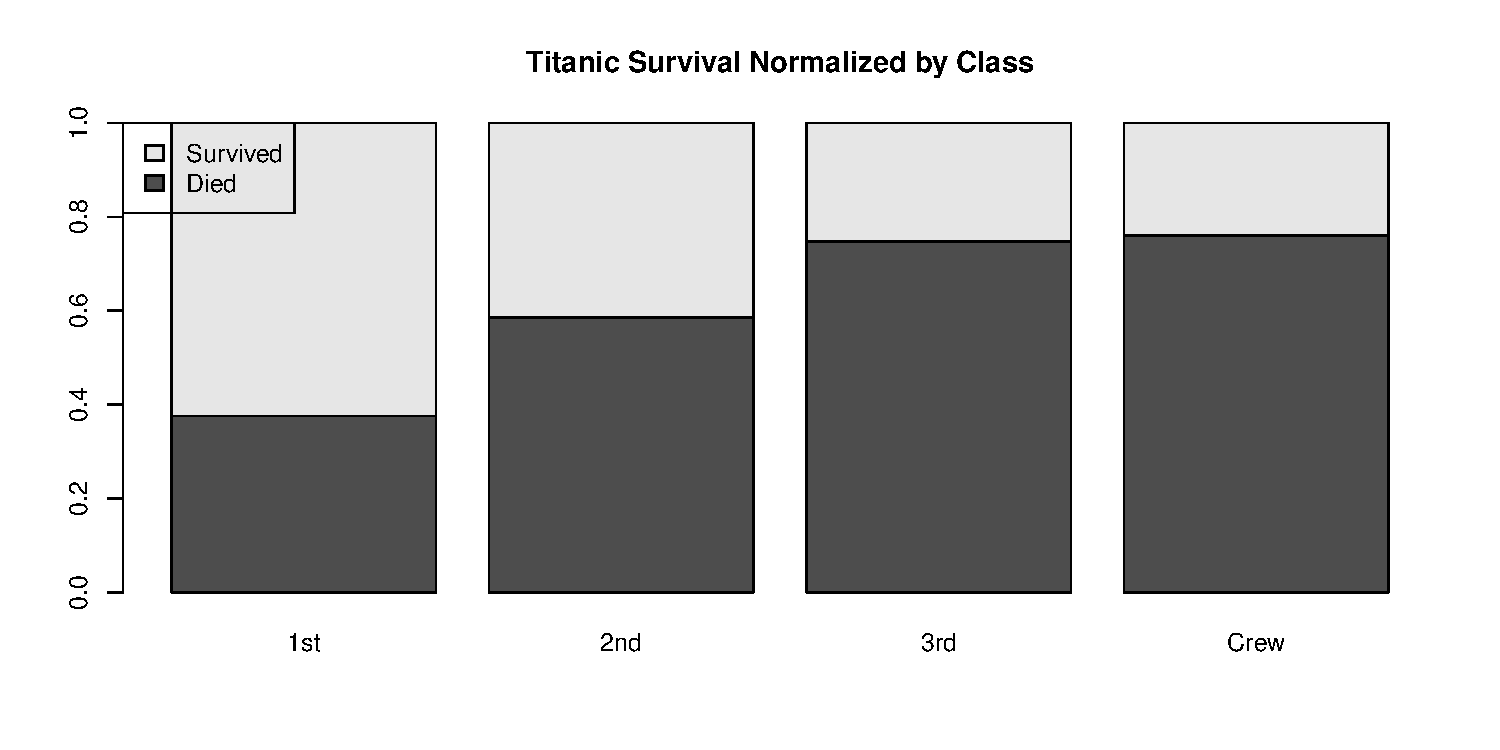
\includegraphics[width=10cm]{figure/norm_barplot.pdf}
%\end{center}
%
%\end{frame}
%%------------------------------------------------------------------------------


%------------------------------------------------------------------------------
\begin{frame}[fragile]
\frametitle{Mosaic Plots}
\blue{Mosaic plots} are similar, but the widths of the bars now reflect proportions:

\begin{center}
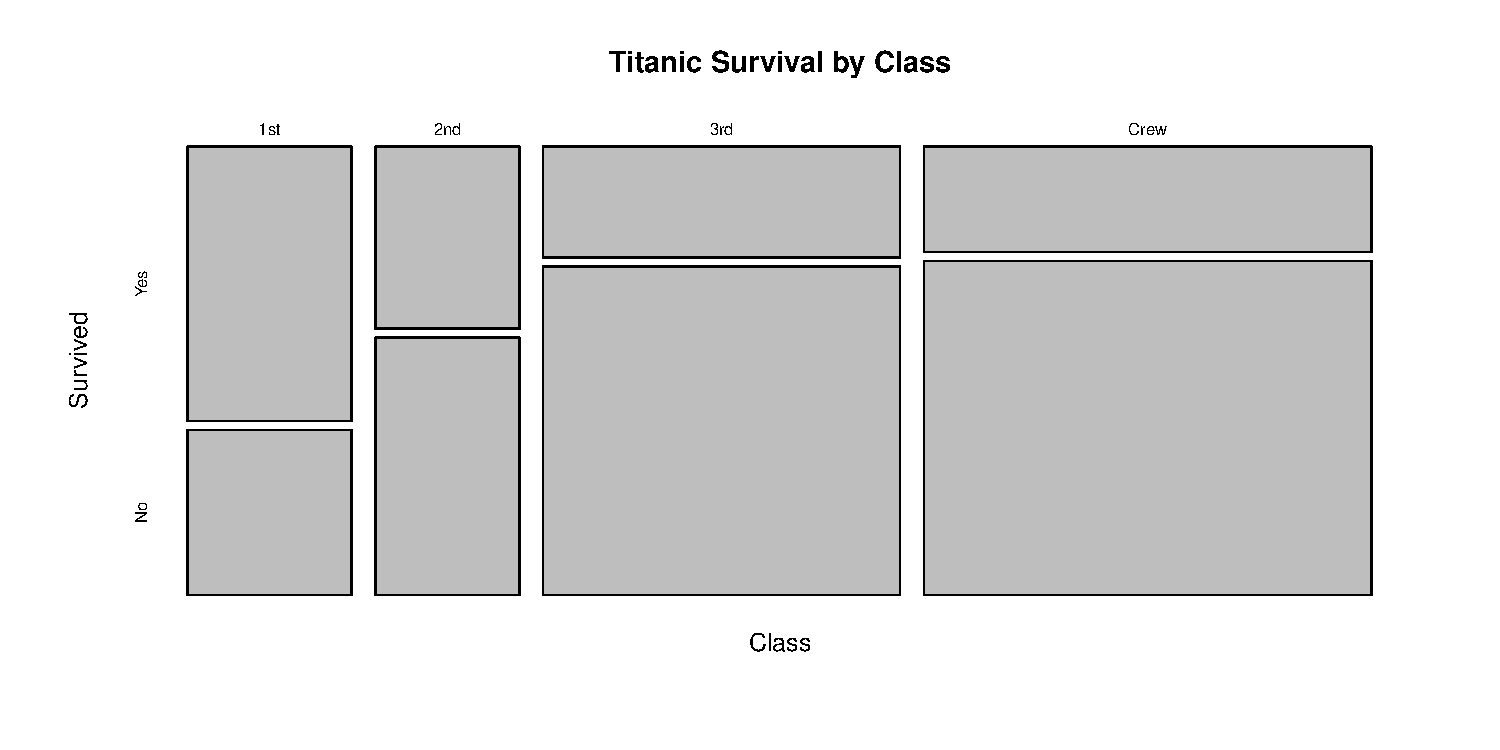
\includegraphics[width=\textwidth]{figure/mosaic_plot.pdf}
\end{center}

\end{frame}
%------------------------------------------------------------------------------


%%------------------------------------------------------------------------------
%\begin{frame}[fragile]
%\frametitle{Further Split on Gender}
%
%\begin{center}
%\begin{tabular}{r|rrrr|r}
%\multicolumn{6}{l}{\blue{Males:}} \\
% & 1st & 2nd & 3rd & Crew & Total \\ 
%  \hline
%Died & 118 & 154 & 422 & 670 & 1364 \\ 
%  Survived & 62 & 25 & 88 & 192 & 367 \\ 
%   \hline
%  Total & 180 & 179 & 510 & 862 & 1731 \\ 
%\end{tabular}
%\end{center}
%  
%\vspace{0.25cm}
%
%\begin{center}
%\begin{tabular}{r|rrrr|r}
%\multicolumn{6}{l}{\blue{Females:}} \\
% & 1st & 2nd & 3rd & Crew & Total \\ 
%  \hline
%Died & 4 & 13 & 106 & 3 & 126 \\ 
%  Survived & 141 & 93 & 90 & 20 & 344 \\
%\hline 
%  Total & 145 & 106 & 196 & 23 & 470 \\ 
%\end{tabular}
%\end{center}
%
%\end{frame}
%%------------------------------------------------------------------------------


%------------------------------------------------------------------------------
\begin{frame}[fragile]
\frametitle{Stacked Barplots}
Using the {\tt ggplot2} package, we can plot survivals by class, age, and gender all at once.

\begin{center}
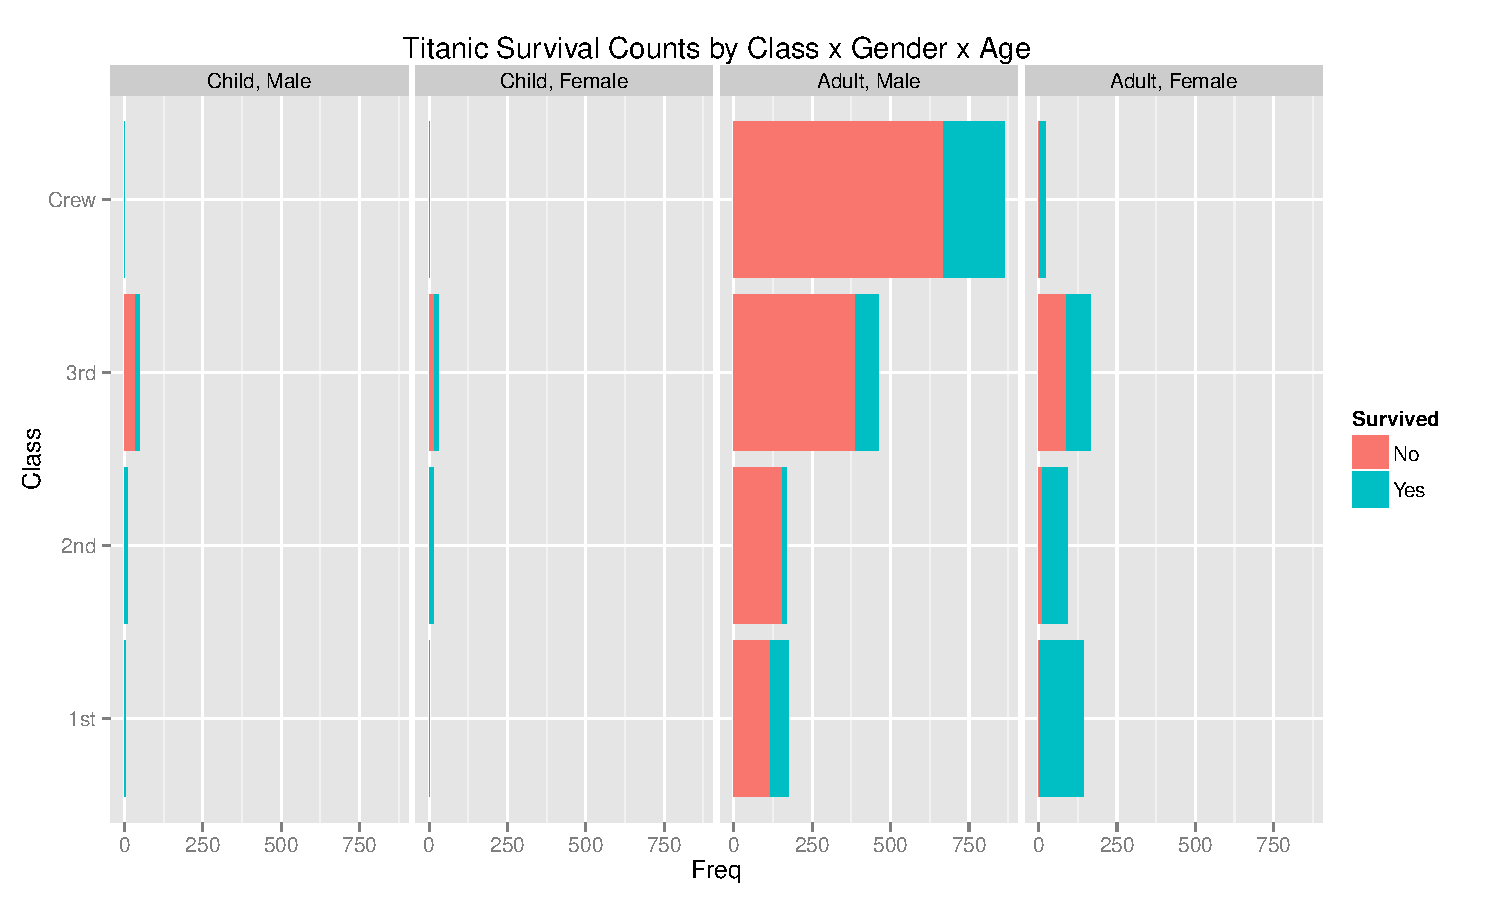
\includegraphics[width=\textwidth]{figure/titanic.pdf}
\end{center}


\end{frame}
%------------------------------------------------------------------------------


%------------------------------------------------------------------------------
\begin{frame}[fragile]
\frametitle{Standardized/Normalized Stacked Barplots}
Instead of raw counts, we can expand each bar to reflect proportions (i.e. standardize/normalize them). 

\begin{center}
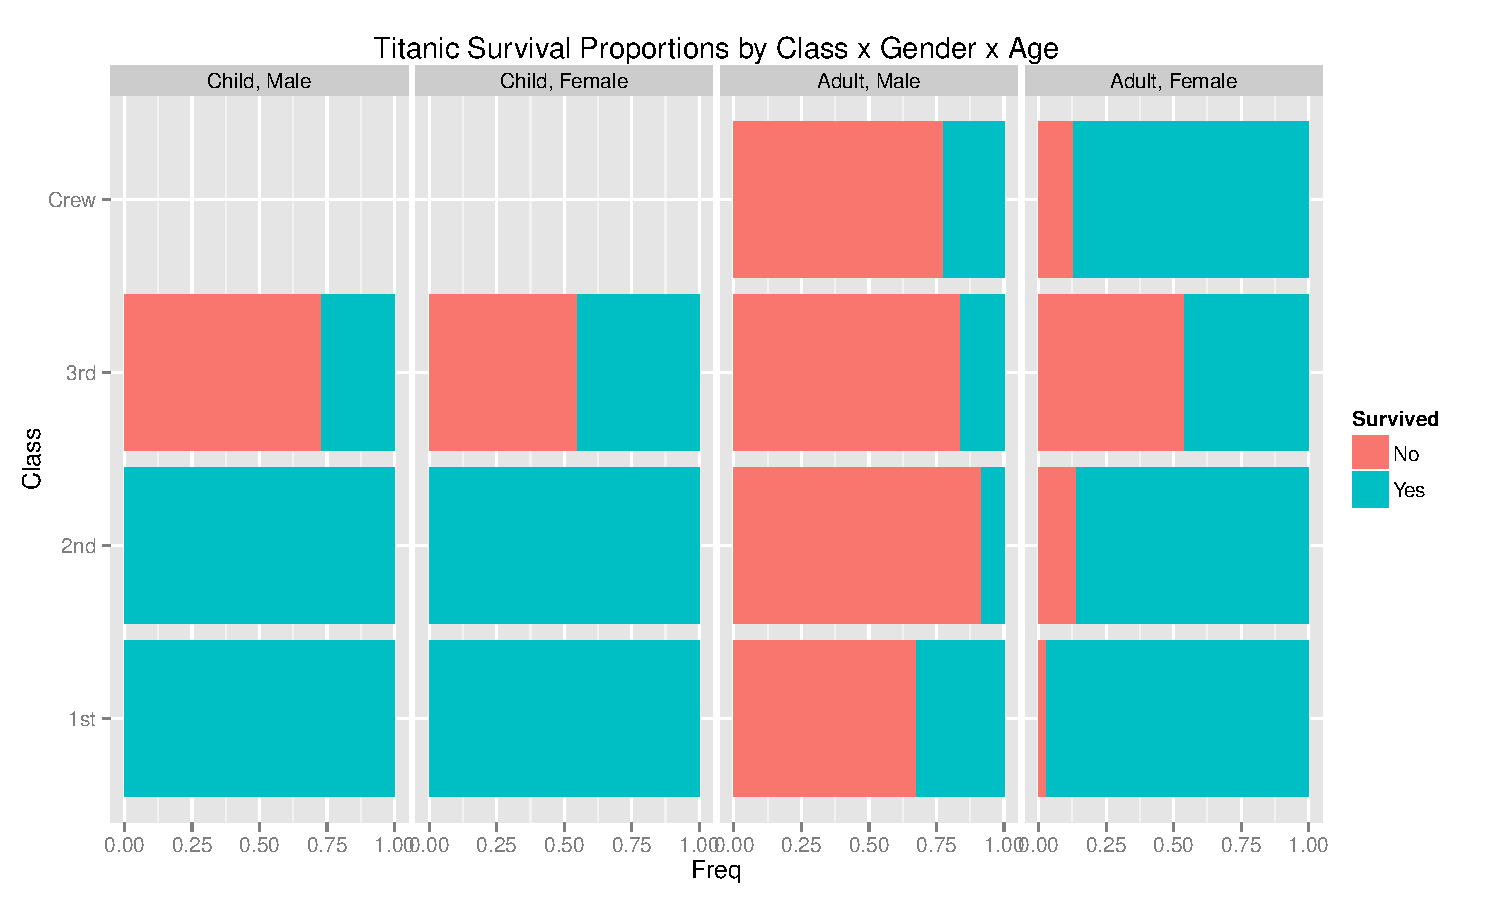
\includegraphics[width=\textwidth]{figure/titanic2.pdf}
\end{center}


\end{frame}
%------------------------------------------------------------------------------


\end{document}










